\documentclass{tufte-handout}
\usepackage{amsmath,amsthm}

%\input{vc.tex}

\usepackage{pgfplots}
\pgfplotsset{width=\textwidth}

\newtheorem{claim}{Claim}[section]
\title{\sf Exact Algorithm for Independent Set}
%\date{\GITAuthorDate, rev. \GITAbrHash}
\author{}

\newcommand{\mis}{\textsc{MIS}}

\begin{document}
\maketitle

\section{Independent Set Lab Report}


by Mats Rydberg and Martin Larsson

\subsection{Correctness}
Algorithm R1 correctly computes $\alpha(G)$ because when we find a node ($a$) with only one neighbour ($b$), we know that either $a$ or $b$ will be in the Maximum Independent Set. What we know is that $a$ has exactly $1$ neighbour while $b$ has \emph{at least} one neighbour. That means that choosing $a$ is always \emph{at least} as good as choosing $b$, so we do that and exclude $b$ from the graph as well.

\noindent
Algorithm R2 correctly computes $\alpha(G)$. If the node we've found ($v$) has two neighbours ($u$, $w$) who are also connected, then this triangle can contribute at most (actually, exactly) $1$ node to the Maximum Independent Set $S$, and so we add $1$ and remove the three. If they are not connected, then we again have two cases: either $1)$ $v$ is in $S$, or $2)$ $u$ and $w$ are \emph{both} in $S$. To accomodate for this difference, and without the need to branch, we introduce $z$. If $v$ is in $S$, $z$ can not be in it since it represents $u$ and $w$ and as such neighbours $v$, and we have not added $1$ too much. If $u$ and $w$ are in $S$, $z$ will also be in it, since none of the nodes bordering $u$ or $w$ can be. So,

$$z = \left\{ \begin{array}{ll}
0 & \Leftrightarrow v \in S \\
1 & \Leftrightarrow u,w \in S \\
\end{array}
\right. $$

\subsection{Empirical Running time}

\paragraph{Experiments.}

\medskip

\noindent
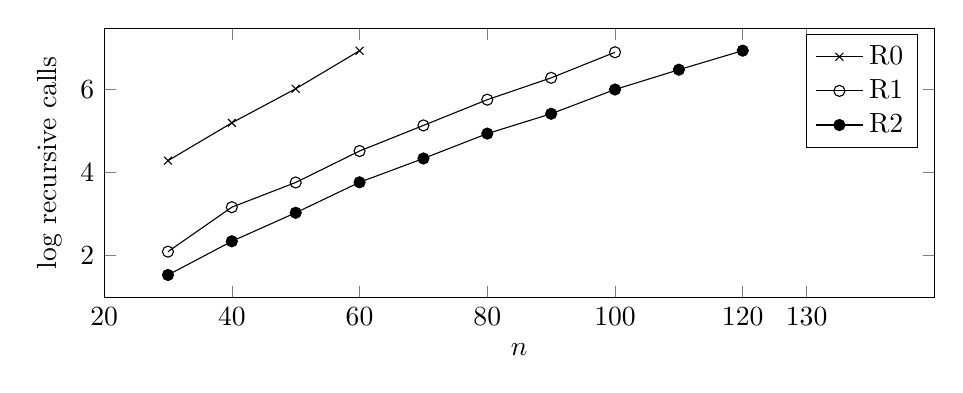
\begin{tikzpicture}
\begin{axis}[
  height= 5cm,
  xlabel=$n$,
  ylabel={log recursive calls},
  xmin = 20,  xmax = 150,
  xtick =       {20,40,60,80,100,120,130},
  xticklabels = { $20$, $40$, $60$, $80$, $100$, $120$, $130$},
  x tick label as interval = false,
  scaled ticks = false
]
    \addplot[color=black, mark=x] 
	coordinates {
	(30, 4.284)
	(40, 5.199)
	(50, 6.024)
	(60, 6.944)
    };
    \addlegendentry{R0}

    \addplot[color=black, mark=o] 
	coordinates {
	(30, 2.083)
	(40, 3.159)
	(50, 3.757)
	(60, 4.518)
	(70, 5.137)
	(80, 5.760)
	(90, 6.288)
	(100, 6.907)
    };
    \addlegendentry{R1}

    \addplot[color=black, mark=*] 
	coordinates {
	(30, 1.519)
	(40, 2.334)
	(50, 3.024)
	(60, 3.761)
	(70, 4.337)
	(80, 4.939)
	(90, 5.419)
	(100, 6.006)
	(110, 6.485)
	(120, 6.946)
    };
    \addlegendentry{R2}


\end{axis}
\end{tikzpicture}
The running times of algorithm~$R_0$, $R_1$, and $R_2$ appear to be
$O(1.3408^n), O(1.1828^n),$ and $O(1.1463^n)$, respectively.

\subsection{Theoretical Upper Bound}

Denote be $T_i(n)$ the worst runtime of algorithm $R_i$ on \emph{any} graph on $n$ vertices.
Note that $T_i(n)$ is a non-decreasing function of $n$.
For $R_0$ we can conclude that
\begin{align*}
T_0(n) &\leq\max(T_0(n-1), T_0(n-1)+T_0(n-1-d_{\mbox{max}})) \\ &\leq T_0(n-1)+T_0(n-2)
\end{align*}
with $d_{\mbox{max}}$ the degree of the vertex we branch on. The hard part is the one when there are no isolated vertices, in which case the vertex $u$ we are branching on has at least one neighbor. 

For R1 we have that
 \[
 T_1(n) \leq T_1(n-1)+T_1(n-3)
 \]

For R2 we have that
 \[
 T_2(n) \leq T_2(n-1)+T_2(n-4)
 \]
\paragraph{Worst Case Upper Bound}
The running times of algorithm~$R_0$, $R_1$, and $R_2$ are in
$O(1.618^n),O(1.466^n),$ and $O(1.380^n)$, respectively.
    
    \newpage

\section{Optional}
Add more ``algorithmic intelligence'' to the algorithm $R_2$ in order to tackle the instance in data/g130.in.
Try to make it run in less than 10,000,000 recursive calls. 

Suggestions for possible speed-ups:
\begin{itemize}
\item Is there some clever (branching) rule for vertices of degree 3?
\item Can we use the information of the largest found independent set so far, to reduce further computation time?
\item What if the graph gets disconnected?
\end{itemize}

\newpage
\section{ Perspective}

This lab establishes medium skills in recursive algorithms implementation,
and simple means to analyze their running time.

\bigskip

The algorithms investigated here can hardly be called ``advanced'', but the main message 
is that no one knows how to do significantly better with any other means.
Indeed, the strongest theoretical worst case run time bound for maximum independent set to date
is obtained by a computerized calculation on a huge set of branching reduction rules, just like the ones we've looked at here [Robson. Algorithms for maximum independent sets. Journal of Algorithms, 7(3):425--440, 1986]. For a much cleaner analysis with just a few rules, obtaining a comparative bound, see [Fomin, Grandoni, and Kratsch. A measure \& conquer approach for the analysis of exact algorithms, JACM 56 (5), article No. 25, 2009].


\end{document}